\documentclass[11pt]{article}
\usepackage{tikz}
\usetikzlibrary{shadows,arrows,positioning}
% Define the layers to draw the diagram
\pgfdeclarelayer{background}
\pgfdeclarelayer{foreground}
\pgfsetlayers{background,main,foreground}
\pagenumbering{gobble}

% Define block styles
\tikzstyle{process} = [draw, fill=blue!20, text centered, text width=12em, minimum width=8em, minimum height=3em, rounded corners, drop shadow,font=\bfseries]
\tikzstyle{inputdata} = [draw, fill=green!20, text centered, text width=12em, minimum width=8em, minimum height=3em, drop shadow,font=\bfseries]
\tikzstyle{tmpdata} = [draw, fill=orange!20, text centered, text width=12em, minimum width=8em, minimum height=3em, drop shadow,font=\bfseries]
\tikzstyle{outputdata} = [draw, fill=red!20, text centered, text width=12em, minimum width=8em, minimum height=3em, drop shadow,font=\bfseries]
\tikzstyle{arrow} = [draw, ultra thick, color=black!50, -latex']
\tikzstyle{line} = [draw, ultra thick, color=black!50, -latex']
\tikzstyle{dash} = [dotted, draw, ultra thick, color=black!50, -latex']
\tikzstyle{layer} = [draw, fill=blue!20, text centered, text width=\linewidth, minimum width=8em, minimum height=3em, rounded corners, drop shadow,font=\bfseries]

% Define distances for bordering
\newcommand{\blockdist}{1.3}
\newcommand{\edgedist}{1.5}
\newcommand{\inputdata}[2]{node (i#1) [inputdata] {#2}}
\newcommand{\tmpdata}[2]{node (t#1) [tmpdata] {#2}}
\newcommand{\outputdata}[2]{node (o#1) [outputdata] {#2}}
\newcommand{\process}[2]{node (p#1) [process] {#2}}
\newcommand{\layer}[2]{node (l#1) [layer] {#2}}


% Draw background
\newcommand{\background}[7]{%
\begin{pgfonlayer}{background}
% Left-top corner of the background rectangle
\path (#1.west |- #2.north)+(-0.5,0.25) node (a1) {};
% Right-bottom corner of the background rectanle
\path (#3.east |- #4.south)+(+0.5,-0.25) node (a2) {};
% Draw the background
\path[fill=#6!20,rounded corners, draw=black!50, dashed] (a1) rectangle (a2);
\path (#3.east |- #2.north)+(0,0.25)--(#1.west |- #2.north) node[midway] (#5-n) {};
\path (#3.east |- #2.south)+(0,-0.35)--(#1.west |- #2.south) node[midway] (#5-s) {};
\path (#3.east |- #2.north)+(0.7,0)--(#3.east |- #4.south) node[midway] (#5-w) {};
% Write test
\node[below of=#4,node distance = 1.3cm, text centered, text width=12em, minimum width=8em, minimum height=3em,font=\bfseries] (tmp) {#7};
\end{pgfonlayer}}

\begin{document}
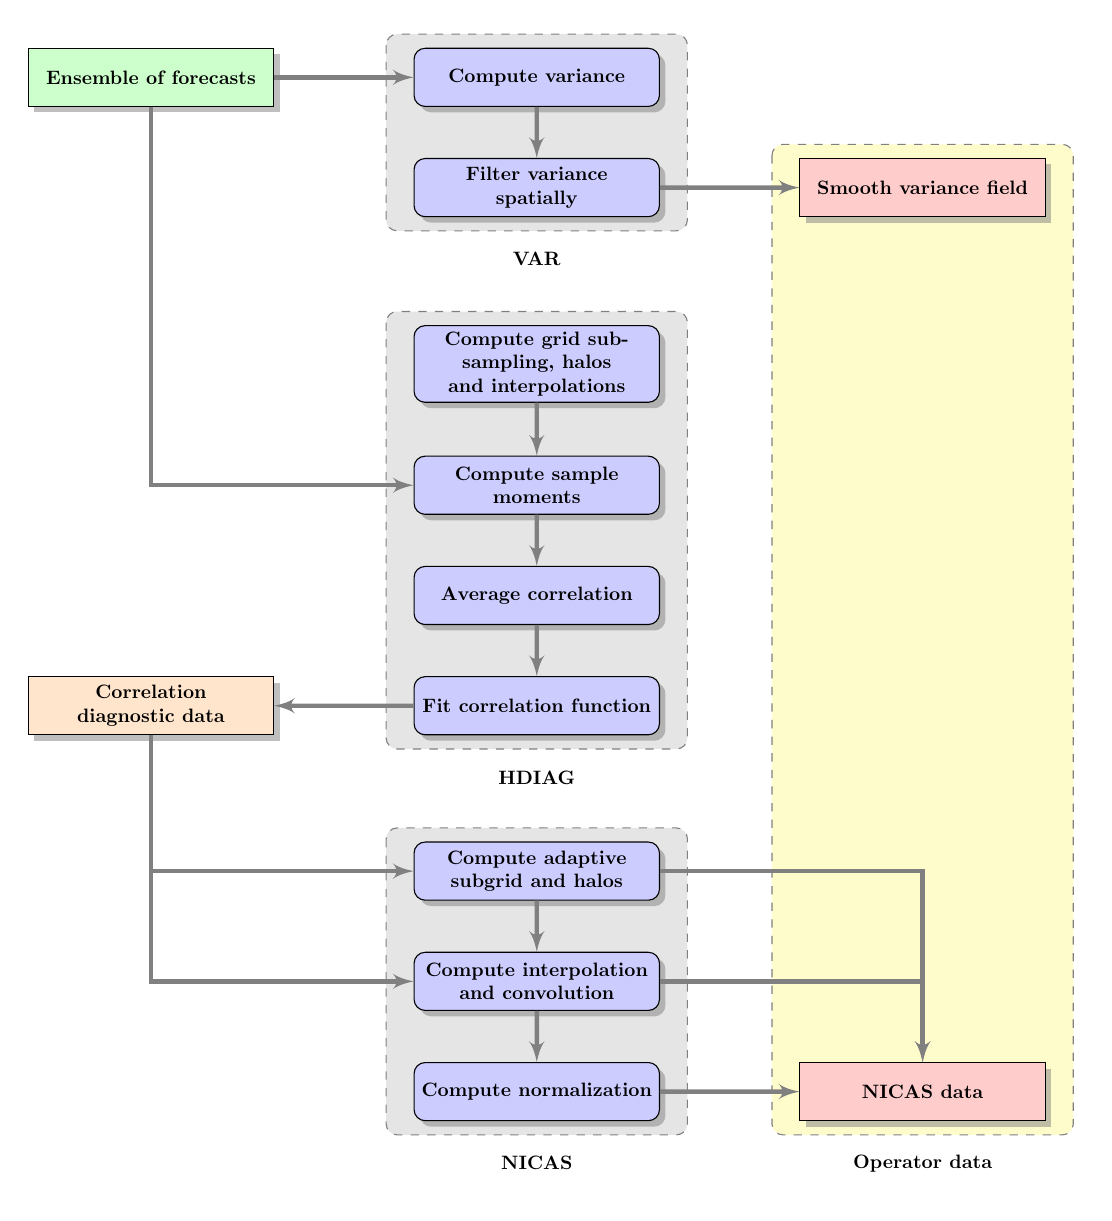
\begin{tikzpicture}[scale=0.7,transform shape]
\path \inputdata{1}{Ensemble of forecasts};
\path (i1)+(7.0,0.0) \process{1}{Compute variance};
\path [arrow] (i1.east) -- (p1.west) node[] {};
\path (p1)+(0.0,-2.0) \process{2}{Filter variance\\ spatially};
\path [arrow] (p1.south) -- (p2.north) node[] {};
\path (p2)+(7.0,0.0) \outputdata{1}{Smooth variance field};
\path [arrow] (p2.east) -- (o1.west) node[] {};

\path (i1)+(7.0,-5.2) \process{3}{Compute grid subsampling, halos and interpolations};
\path (p3)+(0.0,-2.2) \process{4}{Compute sample\\ moments};
\path [arrow] (p3.south) -- (p4.north) node[] {};
\path [arrow] (i1.south) |- (p4.west) node[] {};
\path (p4)+(0.0,-2.0) \process{5}{Average correlation};
\path [arrow] (p4.south) -- (p5.north) node[] {};
\path (p5)+(0.0,-2.0) \process{6}{Fit correlation function};
\path [arrow] (p5.south) -- (p6.north) node[] {};
\path (p6)+(-7.0,0.0) \tmpdata{2}{Correlation\\ diagnostic data};
\path [arrow] (p6.west) -- (t2.east) node[] {};
\path (t2)+(7.0,-3.0) \process{7}{Compute adaptive subgrid and halos};
\path [arrow] (t2.south) |- (p7.west) node[] {};
\path (p7)+(0.0,-2.0) \process{8}{Compute interpolation and convolution};
\path [arrow] (p7.south) -- (p8.north) node[] {};
\path [arrow] (t2.south) |- (p8.west) node[] {};
\path (p8)+(0.0,-2.0) \process{9}{Compute normalization};
\path [arrow] (p8.south) -- (p9.north) node[] {};
\path (p9)+(7.0,0.0) \outputdata{2}{NICAS data};
\path [arrow] (p7.east) -| (o2.north) node[] {};
\path [arrow] (p8.east) -| (o2.north) node[] {};
\path [arrow] (p9.east) -- (o2.west) node[] {};

\background{p1}{p1}{p2}{p2}{bk1}{gray}{VAR}
\background{p3}{p3}{p6}{p6}{bk2}{gray}{HDIAG}
\background{p7}{p7}{p9}{p9}{bk3}{gray}{NICAS}
\background{o1}{o1}{o2}{o2}{bk4}{yellow}{Operator data}
\end{tikzpicture}
\end{document}
